\documentclass[10p,a4paper]{article}
\usepackage[utf8]{inputenc}
\usepackage[T1]{fontenc,url}
\usepackage{multicol}
\usepackage{parskip}
\usepackage{lmodern}
\usepackage{microtype}
\usepackage{verbatim}
\usepackage{amsmath, amssymb}
\usepackage{tikz}
\usepackage{physics}
\usepackage{mathtools}
\usepackage{algorithm}
\usepackage{algpseudocode}
\usepackage{listings}
\usepackage{enumerate}
\usepackage{graphicx}
\usepackage{float}
\usepackage{hyperref}
\usepackage{siunitx}
\usepackage[a4paper, margin=2.5cm]{geometry}
%\setlength\parindent{0pt}

\newcommand{\pptw}{\frac{\partial \Psi}{\partial t}}
\renewcommand{\exp}{e^}
\newcommand{\half}{\frac{1}{2}}

\begin{document}

\subsection*{Random}
$\kappa = \frac{\sqrt{-2mE}}{\hbar}$

Bohr radius: $a = \frac{4\pi\epsilon_0\hbar^2}{me^2} = \SI{0.529e-10}{m}$

Fotonbølgelengde ved elektronhopp: $\frac{1}{\lambda} = \frac{ke^2}{2ahc}\qty(\frac{1}{n_1}-\frac{1}{n_2})$

\textbf{Konstanter:}\\
$hc = \SI{1240}{eV.nm}$\\
$\hbar c = \SI{197.3}{eV.nm}$\\
$m_e = \SI{0.511}{MeV/c^2}$


\section*{Formalisme (kap3+komp.)}
\textbf{Deterministisk tilstand:} Tilstand med en skarpt bestemt målbar størrelse $q$. For eksempel er stasjonære tilstander deterministiske med hensyn på energi (tidløs schrödinger).

\subsection*{Hammiltonrom}
\textbf{Indreprodukt:}$\bra{f(x)}\ket{g(x)} = \int\limits_{-\infty}^\infty f(x)^*g(x) dx$

$\bra{f}\ket{g} = \bra{g}\ket{f}^*$
\\

Komplett sett av $f_n$'er: $f(x) = \sum\limits_{n=1}^\infty c_n f_n(x)$ for vilkårlig $f(x)$.

$c_n$ gitt ved Fouriers triks: $c_n = \bra{f_n}\ket{f}$

\subsection*{Operatorer}
Hermittisk operator(observabel) $\hat{Q}$: $\bra{\Psi_i}\ket{\hat{Q}\Psi_j} = \bra{\hat{Q}\Psi_i}\ket{\Psi_j}$
\\

En observabel størrelse $Q$ representeres ved en operator $\hat{Q}$. De mulig målingene av $Q$ er egenverdiene ($\hat{Q}\psi = q\psi$). Etter måling av en egenverdi $q_n$, vil tilstanden være i den tilhørende egentilstanden(egenvektoren) $\psi_n$.
\\

Egentilstandene, $\psi_n$ utgjør en ortonormal basis av Hammiltonrommet. Vi kan derfor skrive en tilstand som en lin.komb. av egentilstandene til en operator:

$\Psi(x,t) = \sum c_n \psi_n(x) \phi_n(t)$

$|c_n|^2$ er sannsynligheten for å ende med en tilstand $\psi_n$ etter målingen.

$c_n$ finnes ved \textbf{Fouriers triks}:

$c_n = \bra{\psi_n}\ket{\psi} = \int \psi_n(x)^* \psi(x) dx$
\\

\textbf{Forventningsverdi} til operator(ex: energi): $\langle \hat{H} \rangle = \sum\limits_{n=1}^\infty |c_n|^2E_n$
\\

\textbf{Diskret egenverdier:} Dersom egenverdiene/vektorene til en observabel ikke er et kontinuerlig spektra, er egenverdiene $q$ reelle, egenvektorene ligger i Hilbertrommet(normaliserbare), og er ortogonale. F.eks. er harmonisk og inf.square. diskret, mens fripartikkel er kontinuerlig.
\\

\textbf{Kinetisk energi-operator:} $\hat{K} = 0.5m\hat{v}^2 = \frac{\hat{p}^2}{2m}$



\subsection*{Bølge/partikkel relasjoner}

\textbf{Gruppe/fase-hastighet:} $v_g = \frac{d\omega(k)}{dk}$, $v_f = \frac{\omega}{k}$

\textbf{de Broglie's formel:} $p = \frac{2\pi\hbar}{\lambda} = \hbar k$

\textbf{Energi/frekvens:} $E = 2\pi\hbar\nu = \hbar\omega$


\subsection*{Uskarphetsrelasjoner}
$\sigma_A^2\sigma_B^2 \geq \qty(\frac{1}{2i}\langle [\hat{A},\ \hat{B}]\rangle )^2$,
\quad $[\hat{A},\ \hat{B}] = \hat{A}\hat{B} - \hat{B}\hat{A}$, \quad $\sigma_x\sigma_p \geq \frac{\hbar}{2}$



\section*{Kapittel 1 - Statistikk}

\textbf{Forventningsverdien} til $f(j)$ fra en fordeling $P(j)$:

> Diskret j: $\expval{f(j)} = \sum f(j) P(j)$

> Konitnuerlig x: $\expval{f(x)} = \int f(x) p(x) dx$
\\

\textbf{Forv. til operator (sandwitch):} $\expval{Q} = \bra{\Psi}\ket{Q\Psi} = \int \Psi^* (Q) \Psi dx$
\\

\textbf{Standardavvik:} $\sigma = \sqrt{\expval{x^2} - \expval{x}^2}$
\\

\textbf{Normalisering:} $\int |\Psi(x,t)|^2 dx = \int |\Psi^*\Psi| dx = 1$
\\

\textbf{Momentum operator:} $p = -i\hbar\nabla$
\\

\textbf{(Compton-bølgelengde):} $\lambda_c = \frac{h}{mc}$




\section*{Schrödingerligningen}

\textbf{Hammilton:} $\hat{H} = -\frac{\hbar^2}{2m}\nabla^2 + V$\\
(kinetisk + potensiell)
\\

\textbf{Tidløs:} $\hat{H}\psi = E\psi$ (egenverdi/vektor lign. for H)

$\Psi(x,t) = \sum \Psi_n(x,t) = \sum c_i \psi_n(x)\varphi(t)$

$\varphi(t) = \exp{-iE_nt/\hbar}$

Fouriers triks: $c_n = \bra{\psi_n}\ket{\psi}$
\\

\textbf{Tidsavhengig:} $\hat{H}\Psi = i\hbar\pptw$
\\

Tidskomponenten $\phi(t)$ av bølgeligningen er eksplisitt definert av energinivået. Den romlige komponenten $\phi(x)$ må løses implisitt av schrödingerligningen.




\section*{1D - Spesifikke potensialer}

\subsection*{Uendelig potensialbrønn}
$\psi_n(x) = \sqrt{\frac{2}{a}}\sin(\frac{n\pi}{a}x)$ \quad\quad (ortogonale løsn.)

$E_n = \frac{n^2\pi^2\hbar^2}{2ma^2}$


\subsection*{Harmonisk oscilator}
$V(x) = 1/2kx^2 = 1/2m\omega^2x^2$ \hspace{1cm} $E_n = \qty(n+\half)\hbar\omega$

$\psi_0(x) = \qty(\frac{m\omega}{\pi\hbar})^{1/4}\exp{-m\omega x^2 / 2\hbar}$ \hspace{1cm} $\psi_n(x) = A_n (a_+)^n \psi_0(x)$

$a_{\pm} = \frac{1}{\sqrt{2\hbar m \omega}}(\mp ip + m\omega x)$
\\

Husk: Eneste som begynner på $n=0$.


\subsection*{Fri partikkel}
Fripartikkelløsningene er en vektet sum av et spekter av planbølgeløsninger med forskjellig bølgetall(bølgelengde) $k$. For et kontinuerlig spekter av $k$ blir dette et integral.

$\Psi(x,t) = \frac{1}{\sqrt{2\pi}}\int\limits_{-\infty}^\infty\phi(k)\Psi_k(x,t) dk$ 
\\

Separable planbølgesløsninger(ikke normaliserbare):\\
$\Psi_k(x,t) = A\exp{i(kx-\frac{\hbar k^2}{2m}t)}$ \hspace{1cm} $k = \pm \frac{\sqrt{2mE}}{\hbar}$

Koeffisienter: $\phi(k) = \frac{1}{\sqrt{2\pi}}\int\limits_{-\infty}^\infty\phi(x,0)\exp{-ikx} dk$





\section*{3D - Sfæriske koordinater}
\textbf{Separable løsninger:}\\
Vi seprarer mellom de radielle og angulære løsningene.
\[ \Psi_{nlm}(r, \theta, \psi) = R_{nl}(r)Y_l^m(\theta, \psi) \]

\textbf{Radiell schrö:}\\
De radielle løsningene er definert av den radielle scrödingerligningen, som minner om den 1 dimensjonale, bare med et spinn-ledd på potensialet.
\begin{align*} \hat{H}u = Eu \hspace{1.2cm} u(r) = rR(r)\\
\hat{H} = -\frac{\hbar^2}{2m}\frac{d^2}{dr^2} + \qty[V + \frac{\hbar^2}{2m}\frac{l(l+1)}{r^2}]\end{align*}

\textbf{Angulær shcrö: (sfærisk harmoniske)}\\
De angulære løsningene er eksplisitt definert.
\[ Y_l^m(\theta, \phi) = A\Phi(\phi)\Theta(\theta) = \epsilon\sqrt{\frac{2l+1}{4\pi}\frac{(l-|m|)!}{(l+|m|)!}} e^{im\phi} P_l^m(\cos(\theta)) \]

\textbf{Legendre function:} $P_l^m(x) = (1-x^2)^{|m|/2} \qty(\frac{d}{dx})^{|m|} P_l(x)$

\textbf{Legendre polynomials:} $P_l(x) = \frac{1}{2^ll!}\qty(\frac{d}{dx})^l (x^2-1)^l$
\\

\textbf{Indreprodukt i sfæriske koordinater:}
\[ \bra{f(r,\theta,\phi)}\ket{g(r,\theta,\phi)} = \int\limits_0^{2\pi}\int\limits_0^\pi\int\limits_0^\infty f(r,\theta,\phi)^*g(r,\theta,\phi)\ r^2\sin\theta dr d\theta d\phi \]

\textbf{Normalisering:}
\begin{align*}
\int\limits_0^\infty |R|^2r^2 dr = \int\limits_0^{2\pi}\int\limits_0^\pi |Y|^2\sin\theta d\theta d\phi = 
\int\limits_0^{2\pi}\int\limits_0^\pi\int\limits_0^\infty |\Psi|^2 r^2\sin\theta dr d\theta d\phi = 1
\end{align*}

\textbf{Sfærisk harmoniske:}

$
Y_0^0(\theta, \phi) = \frac{1}{2}\sqrt{\frac{1}{\pi}}
\\
Y_1^{-1}(\theta, \phi) = \frac{1}{2}\sqrt{\frac{3}{2\pi}} \cdot \exp{-i\phi} \cdot \sin\theta
\\
Y_1^0(\theta, \phi) = \frac{1}{2}\sqrt{\frac{3}{\pi}} \cdot \cos\theta
\\
Y_1^1(\theta, \phi) = -\frac{1}{2}\sqrt{\frac{3}{2\pi}} \cdot \exp{i\phi} \cdot \sin\theta
\\
Y_2^{-2}(\theta, \phi) = \frac{1}{4}\sqrt{\frac{15}{2\pi}} \cdot \exp{-2i\phi} \cdot \sin^2\theta
\\
Y_2^{-1}(\theta, \phi) = \frac{1}{2}\sqrt{\frac{15}{2\pi}} \cdot \exp{-i\phi} \cdot \sin\theta \cdot \cos\theta
\\
Y_2^0(\theta, \phi) = \frac{1}{4}\sqrt{\frac{5}{\pi}} \cdot (3\cos^2\theta - 1)
\\
Y_2^1(\theta, \phi) = -\frac{1}{2}\sqrt{\frac{15}{2\pi}} \cdot \exp{i\phi} \cdot \sin\theta \cdot \cos\theta
\\
Y_2^2(\theta, \phi) = \frac{1}{4}\sqrt{\frac{15}{2\pi}} \cdot \exp{2i\phi} \cdot \sin^2\theta
\\
Y_3^{-3}(\theta, \phi) = \frac{1}{8}\sqrt{\frac{35}{\pi}} \cdot \exp{-3i\phi} \cdot \sin^3\theta
\\
Y_3^{-2}(\theta, \phi) = \frac{1}{4}\sqrt{\frac{105}{2\pi}} \cdot \exp{-2i\phi} \cdot \sin^2\theta \cdot \cos\theta
\\
Y_3^{-1}(\theta, \phi) = \frac{1}{8}\sqrt{\frac{21}{\pi}} \cdot \exp{-i\phi} \cdot \sin\theta \cdot (5\cos^2\theta - 1)
\\
Y_3^0(\theta, \phi) = \frac{1}{4}\sqrt{\frac{7}{\pi}} \cdot (5\cos^3\theta - 3\cos\theta)
\\
Y_3^1(\theta, \phi) = -\frac{1}{8}\sqrt{\frac{21}{\pi}} \cdot \exp{i\phi} \cdot \sin\theta \cdot (5\cos^2\theta - 1)
\\
Y_3^2(\theta, \phi) = \frac{1}{4}\sqrt{\frac{105}{2\pi}} \cdot \exp{2i\phi} \cdot \sin^2\theta \cdot \cos\theta
\\
Y_3^3(\theta, \phi) = -\frac{1}{8}\sqrt{\frac{35}{\pi}} \cdot \exp{3i\phi} \cdot \sin^3\theta
$



\subsection*{Hydrogen}
Rad.Schrö: $\frac{d^2u}{dr^2} = \qty[1-\frac{\rho_0}{\rho} + \frac{l(l+1)}{\rho^2}]u$
\hspace{0.6cm}$\rho = \kappa r$,\hspace{0.6cm} $\rho_0 = \frac{me^2}{2\pi\epsilon_0\hbar^2\kappa}$

$E_n = -\qty[\frac{m}{2\hbar^2}\qty(\frac{e^2}{4\pi\epsilon_0})^2]\frac{1}{n^2} = \frac{E_1}{n^2}$

Løsninger: $\Psi_{nlm} = R_{nl}Y_{lm}$

$R_{nl} = \sqrt{\qty(\frac{2}{na})^3\frac{(n-l-1)!}{2n[(n+l)!]^3}}\exp{-r/na}\qty(\frac{2r}{na})^l L_{n-l-1}^{2l+1}\qty(\frac{2r}{na})$




\subsection*{Angulærmoment}
Totalt og komponent- angulærmoment:
\[  L^2 Y_l^m = \hbar^2 l(l+1)Y_l^m \hspace{1cm} L_z Y_l^m = \hbar m Y_l^m\]


\textbf{Asimutalt kvantetall} $l = 0,\ 1,\ 2,\ \dots,\ n-1$.\\
Bestemmer totalt angulærmoment. 
\\

\textbf{Magnetisk kvantetall} $m = -l,\ -l+1,\ \dots,\ l-1,\ l$.\\
Bestemmer orienteringen av angulærmomenten - andelen av angulærmoment i $z$-retning.
\\

\textbf{Identiteter:}
\[L_\pm = L_x \pm i L_y \hspace{1cm} L_z = \frac{\hbar}{i}\frac{\partial}{\partial\phi}\]
\[\hat{L}^2 = -\hbar^2\qty[\frac{1}{\sin\theta}\frac{\partial}{\partial\theta}\qty(\sin\theta\frac{\partial}{\partial\theta}) + \frac{1}{\sin^2\theta}\frac{\partial^2}{\partial\phi^2}]\]
\\
Heve- og senke-operatorene endrer andelen av $L_z$ i $\vec{L}$. Med andre ord, endrer $m$ med 1, som også endrer egenverdien til $L_z$ med $\hbar$.
\\

\textbf{Kommutatorer:} (Gjelder identisk for spinn)
\[  [L^2, \textbf{L}] = 0, \hspace{1cm} [L_x, L_y] = i\hbar L_z\ \dots\]




\subsection*{Spinn}

Innebygget magnetisk \textbf{dipolmoment}:
\[ \vec{\nu_s} = -g_e\frac{e}{2m_e}\vec{S},\quad g_e \approx 2\]

\textbf{Totalspinn} og \textbf{spinnkomponent} i $z$-retning:
\begin{align*}
S = |\vec{S}| &= \hbar\sqrt{s(s+1)} \hspace{1.5cm} S_z = \hbar m_s \\
\hat{S}^2\chi &= \hbar^2s(s+1)\chi \hspace{0.8cm} \hat{S_z}\chi = \hbar m_s \chi
\end{align*}
\\
Vi kaller egenvektorene til spinn for $\chi_{m_s}$, eller $\ket{s\ m_s}$, som er en vektor entydig definert av $s$ og $m_s$
\\

\textbf{Spinnkvantetallet} $s = 0,\ \frac{1}{2},\ 1,\ \frac{3}{2},\dots$\\
Heltall for \textbf{bosoner}(fotoner), halvtall for \textbf{fermioner}(elektroner, protoner, nøytroner). Bestemmer totalspinn.
\\

\textbf{Magnetisk spinnkvantetall} $m_s = -s,\  -s+1,\ \dots \, s-1,\ s$.\\
Bestemmer mengden av totalspinn i $z$-retning.
\\

Bølgeligningen med spinntilstand: $\psi_{nlmm_s} = \psi_{nlm}\chi_{m_s}$
\\

Spinnoperatorer påvirker ikke $\psi_{nlm}$, og romlige operatorer påvirker ikke $\chi_{m_s}$.

\subsection*{Fermioner - Spinn $s = 1/2$}
Alle kjente fermioner har et spinnkvantetall $s = 1/2$. Dette gir to mulige spinntilstander, kalt "spinn opp"($l=1/2$) og "spinn ned"($=-1/2$):
\begin{align*}
\ket{\tfrac{1}{2}\ \tfrac{1}{2}} = \chi_+ = \begin{pmatrix} 1 \\ 0 \end{pmatrix} = \ket{\uparrow}\\
\ket{\tfrac{1}{2}\ \tfrac{-1}{2}} = \chi_- = \begin{pmatrix} 0 \\ 1 \end{pmatrix} = \ket{\downarrow}
\end{align*}

Disse to tilstandene danner en komplett basis for Hilbert rommet, slik at alle spinntilstander kan skrives som lineærkombinasjoner av disse (også spinnet i $x$ og $y$ retning.

Spinn-operatorene blir nå 2x2 matriser, kalt \textbf{Pauli spinn matriser}:
\begin{equation*}
\hat{S}^2 = \frac{3}{4}\hbar^2
\begin{pmatrix}
1 & 0\\
0 & 1
\end{pmatrix} \quad \quad
\hat{S} = \frac{\hbar}{2}\sigma
\end{equation*}

\begin{equation*}
\sigma_x =
\begin{pmatrix}
0 & 1\\
1 & 0
\end{pmatrix}
\sigma_y =
\begin{pmatrix}
0 & -i\\
i & 0
\end{pmatrix}
\sigma_z =
\begin{pmatrix}
1 & 0\\
0 & -1
\end{pmatrix}
\end{equation*}

\begin{equation*}
S_+ = \hbar
\begin{pmatrix}
0 & 1\\
0 & 0
\end{pmatrix}
S_- = \hbar
\begin{pmatrix}
0 & 0\\
1 & 0
\end{pmatrix}
\end{equation*}

\subsection*{Spinnkombinasjoner:}
Når vi kombinerer to $s = 1/2$ partikler i ett system (e.g. elektron + proton i hydrogen, eller elektroner i et atomskall) får vi enten en triplet $s = 1$, eller en singlet $s = 0$. Merk at tripleten er symetrisk, mens singleten er anti-symetrisk.

\begin{align*}
\text{triplet, } s = 1
\begin{cases}
\ket{\uparrow \uparrow} & \ket{1\ 1}\\
\tfrac{1}{\sqrt{2}}(\ket{\uparrow \downarrow} + \ket{\downarrow \uparrow}) & \ket{1\ 0}\\
\ket{\downarrow \downarrow} & \ket{1\ -1}
\end{cases}
\end{align*}

\begin{align*}
\text{singlet, } s = 0
\begin{cases}
\tfrac{1}{\sqrt{2}}(\ket{\uparrow \downarrow} - \ket{\downarrow \uparrow}) & \ket{0\ 0}\\
\end{cases}
\end{align*}

\subsection*{Flerpartikkelsystemer}
Gitt to partikler i tilstandene $\psi_a(r)$ og $\psi_b(r)$. For ikke-identiske(ikke vekselvirkende) partikler er den samlede bølgefunksjon gitt som
\[\psi(r_1, r_2) = \psi_a(r_1)\psi_b(r_2)\]

Dersom partiklene er identiske og vi ikke kan se forskjell på dem er bølgefunksjonen annerledes.
\\

Bosoner har en \textbf{symetrisk bølgefunksjon:}
\[ \psi(r_1,r_2) = A[\psi_a(r_1)\psi_b(r_2) + \psi_b(r_1)\psi_a(r_2)] \]

Fermioner har en \textbf{antisymetrisk bølgefunksjon:}
\[ \psi(r_1,r_2) = A[\psi_a(r_1)\psi_b(r_2) - \psi_b(r_1)\psi_a(r_2)] \]

For fermioner må vi ha en antisymetrisk bølgefunksjon. Dette kan innebære enten en symetrisk romdel og en antisymetrisk spinndel(singlet), eller motsatt.
\\

\textbf{Paulis eksklusjonsprinsipp}\\
To fermioner kan ikke være i samme tilstand $\psi_a = \psi_b$, ettersom den antisymetriske bølgefunksjonen da blir$\psi = 0$. To fermioner kan derfor ikke ha samme sett med kvantetall. Somregel svarer dette til at to fermioner i samme romlige tilstand må ha forskjellig magnetisk kvantetall $m_s$.
\\

\textbf{Degenerasjon:}\\
Et degenerert system er et system der flere tilstander gir samme energinivå. Degenerasjonsgraden $d(n)$ er antallet tilstander som gir samme energinivå for et gitt energikvantetall $n$.

\newpage

\textbf{Fotoelektrisk effekt:} Monokromatisk lys mot metallplate, eletroner blir emmitert og går over til anoden. Spenning bestemmer hvor mange av elektronene som går over til anoden. Resultat: 1. En nedre grense for frekvensen til lyset som gir elektroner(. 2. utsendingen av elektroner var umiddelbar. 3. Kinetisk energi til elektronene var uavhengig av lysintensiteten, og hadde en øvre grense. Dette viste kvantisering av fotoner. Økt lysintensitet gir mer strøm, men ikke større kinetisk energi på elektronene.
\begin{figure}[H]
\centering
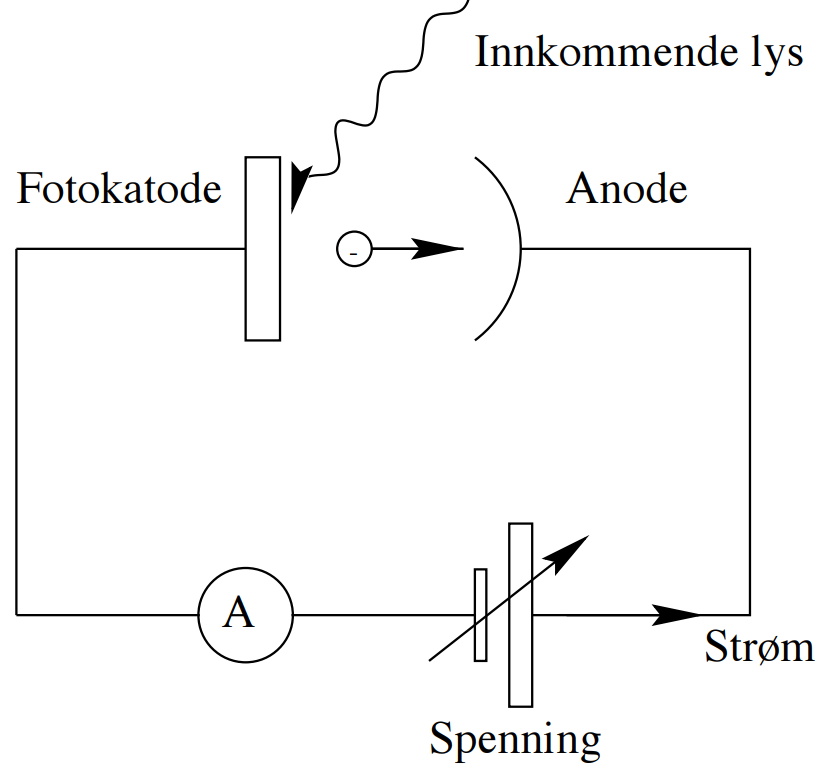
\includegraphics[width=0.2\textwidth]{foto.png}
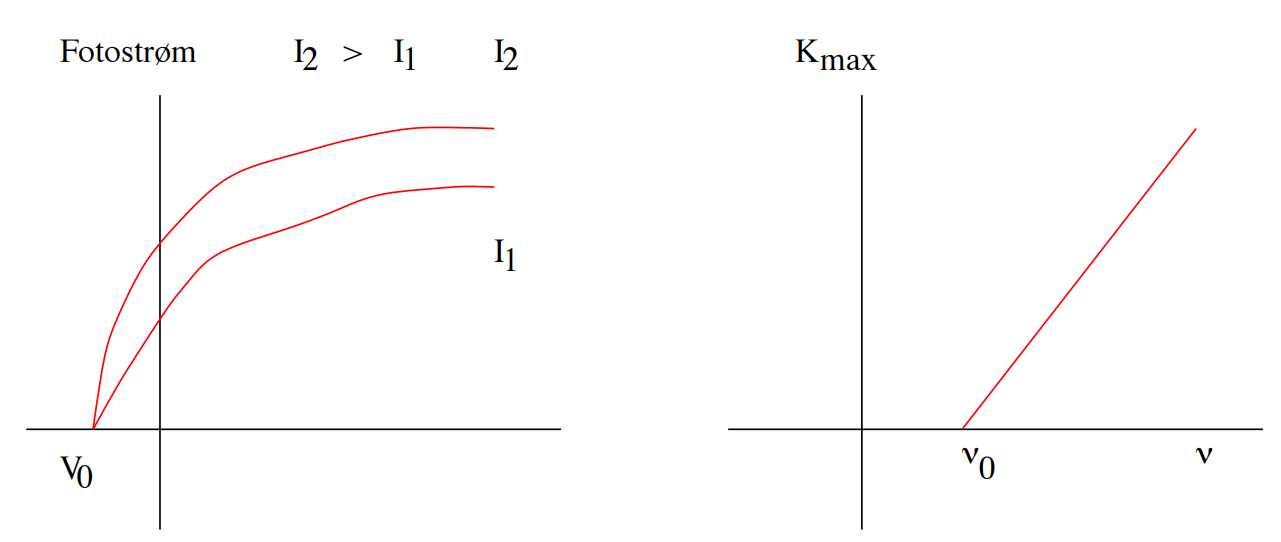
\includegraphics[width=0.4\textwidth]{foto2.png}
\end{figure}


\textbf{Rontgenstråling:} Motsatt av foto. Elektroner akselereres gjennom et spenningsvall $V_R$, og bremses(koliderer) mot en metallplate, og avgir fotoner fordi de deakselereres(bremsstraahlung). Man observerte en maksimal frekvens/energi hos de utsendte fotonene, lik den kinetiske energien til et enkelt elektron $\lambda_{min} = hc/eV_R$. Denne minimale bølgelengden kunne ikke forklares klassisk.
\begin{figure}[H]
\centering
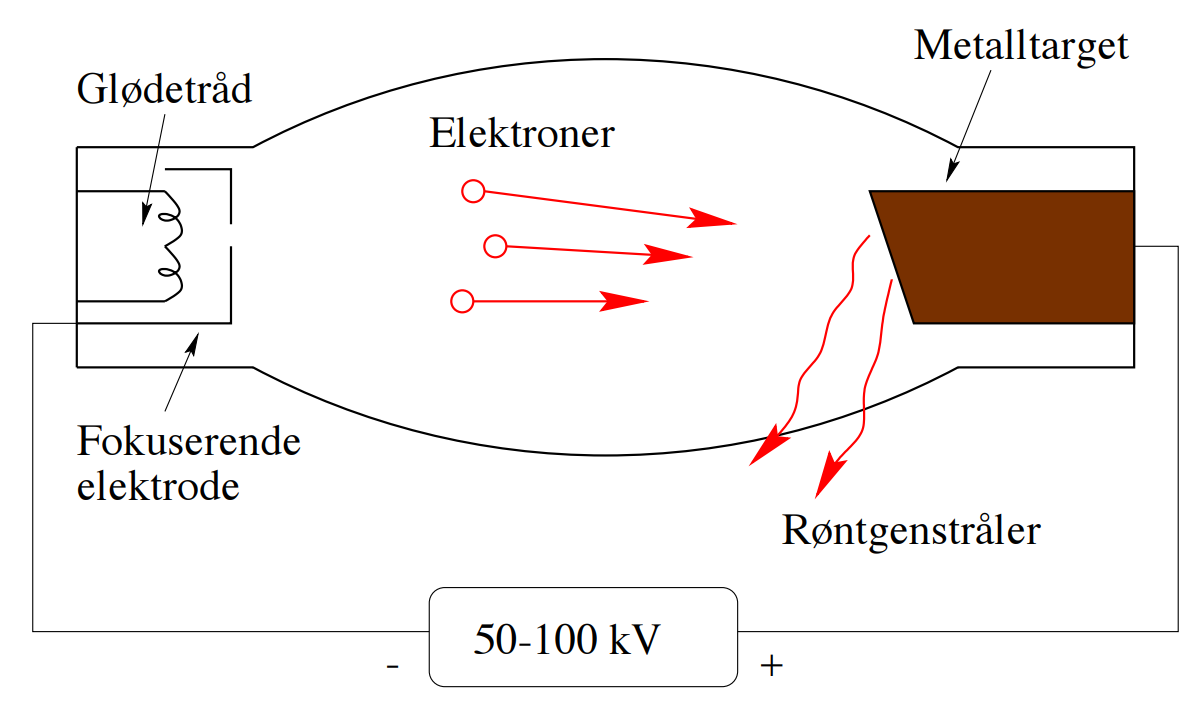
\includegraphics[width=0.3\textwidth]{rontgen.png}
\end{figure}


\textbf{Comptonspredning:} Viste at lys må ha bevegelsesmengde. Foton kolliderer med "fritt" elektron (neglisjerbar arbeidsfunksjon grunnet store energier). Fotonet får høyere bølgelengde (lavere bevegelsesmengde) etter støtet med elektronet. Viser også bølge/partikkel egenskaper: Målingen av de spredte EM-strålene bygger på bølgeteori (Braggdiffraksjon), mens spredningen påvirker bølgelengden på en måte som bare kan forklares ved å se på rontgenstrålen som parikler. Den observerte strålen inneholder også en del av den originale bølgelengden til strålen, som kommer fra fotoner som ikke løsrev elektroner, og hadde en elastisk kollisjon med et atom.
\[ \Delta \lambda = \lambda_C (1-\cos\theta) = \frac{h}{m_ec}(1-\cos\theta) \]

\begin{figure}[H]
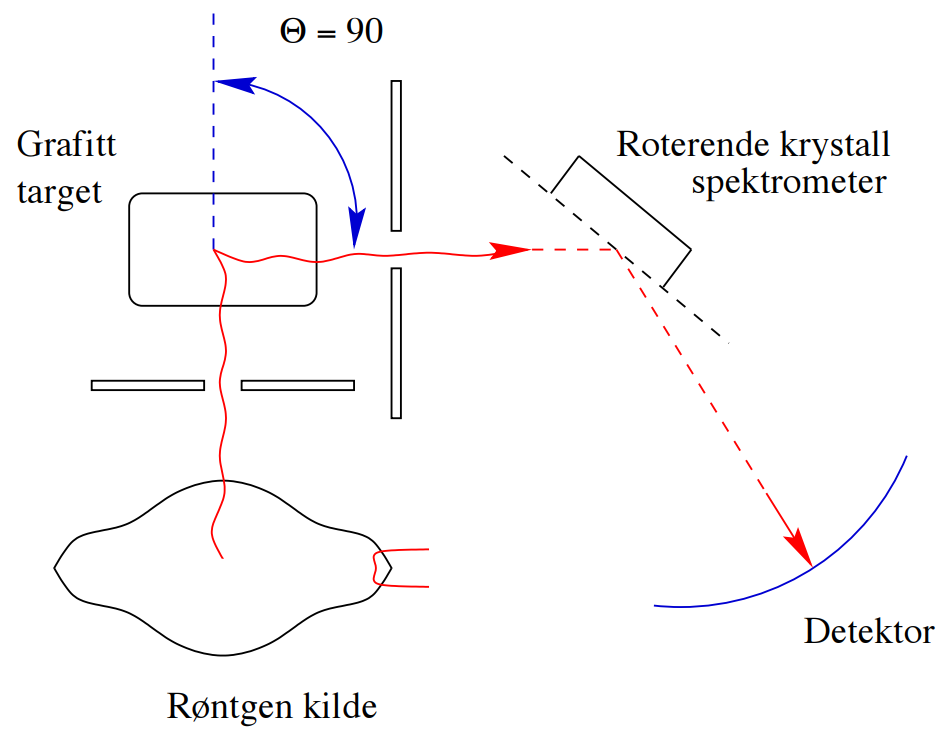
\includegraphics[width=0.25\textwidth]{compton.png}
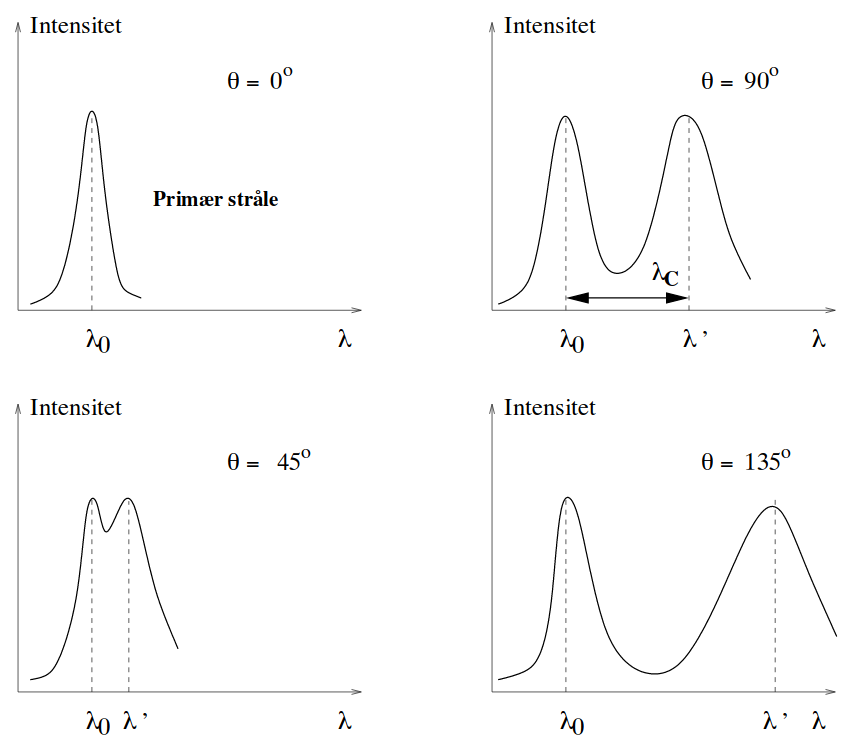
\includegraphics[width=0.25\textwidth]{compton2.png}
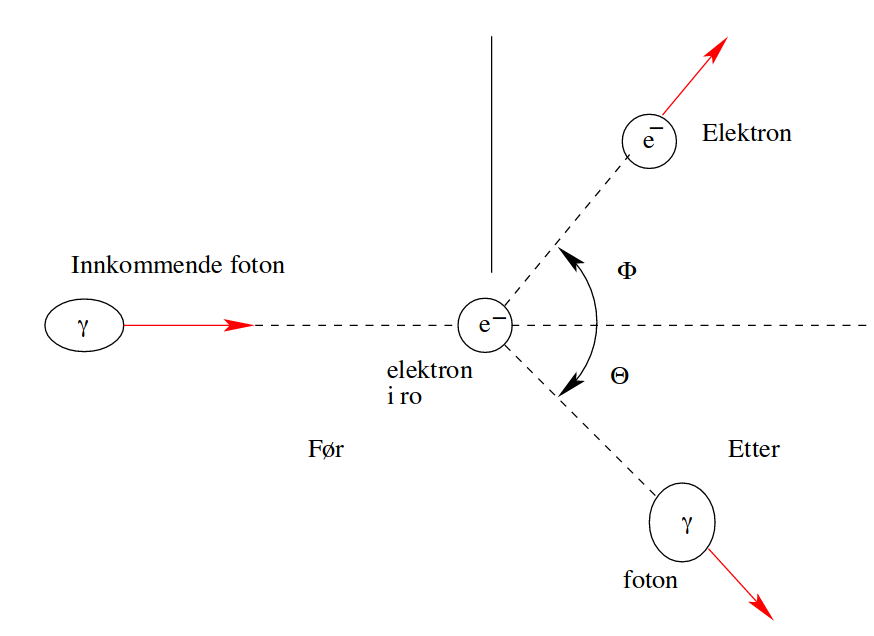
\includegraphics[width=0.3\textwidth]{compton3.png}
\end{figure}


\textbf{Franck-Hertz eksperimentet:} Elektroner akselereres over et spenningsfall fra en katode til et gitter, og deakselereres deretter av en (mindre) spenningsøkning mellom gitteret og anoden. Elektroner som går uhindret kommer til anoden med en kinetisk energi $K_e = e\cdot V_{KA}$, og det går strøm. Elektroner som reagerer med kvikksølvatomene i gassen kommer ikke frem. Det viste seg at når $K_e$ tilsvarte et multiplum av energien til den første eksiterte tilstanden til kvikksølv, falt strømmen. Dette skjedde ved multiplum av $\SI{4.9}{V}$, og beviste Bohrs atommodell med kvantiserte energinivåer.
\begin{figure}[H]
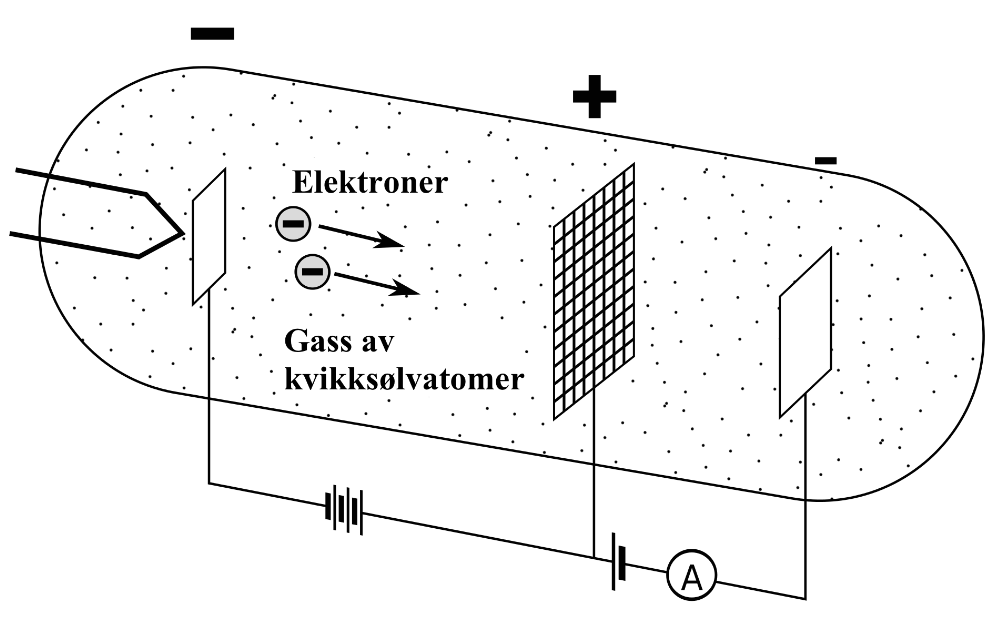
\includegraphics[width=0.25\textwidth]{FranckHertz.png}
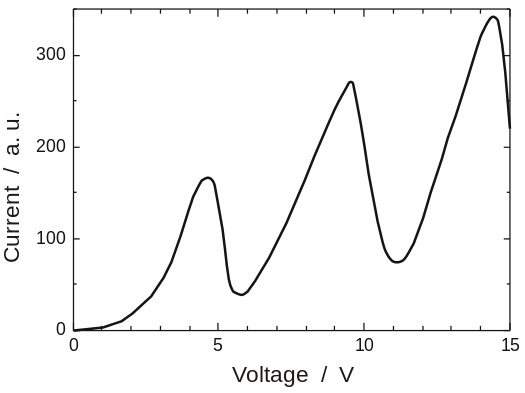
\includegraphics[width=0.2\textwidth]{FranckHertz2.png}
\end{figure}

\textbf{Stern-Gerlach eksperimentet:} To magneter setter opp et inhomogent magnetfelt. Skulle teste om angulærmomentet ($vec{L}$) i hydrogen er kvantisert. Forventer avbøyninger av hydrogen(eller sølv) etter hydrogenatomets dipolmoment:
\[ \vec{\nu} = -\frac{e}{2m_e}\vec{L} \]
Forventet å observere $2l+1$ linjer på skjermen(antall mulige $m$ for en gitt $l$). Man observerte dobbelt så mange(to linjer veldig tett på hverandre for hver linje man forventet). Dette kom av at elektronet også hadde et egenspinn, som også ble litt påvirket av det ytre magnetfeltet.


\end{document}
